%% Paper 1: physics-only exploration of the thermochemical space for neural chemistry surrogates.
%% Draft v0, 2026-11-21 (Spain time). Target: Combustion and Flame (alt. Energy and AI).
%% Sources: chemmanifold/ (stages 0-4, holes.py, unsteady_flamelet.py), configs/burner_openfoam_{ood8,tix2,tix2h,tix2c}.yaml,
%%   papers/data/coverage/, results/sim1/{B,C2,offline_v2}/ (branch claude/project-thread-mq77al), project-file
%%   reports of the OOD loop (bucle-ood/), the exploration explainer (exploracion/) and the hole analysis (huecos-cobertura/).
%% Figures: figs/0*.png and 1*.png from exploracion/figures/make_figs.py; fig_coverage/fig_families from scripts/make_figs.py.
%% \todo{} = must be resolved before submission.
\documentclass[preprint,review,12pt]{elsarticle}

\usepackage[T1]{fontenc}
\usepackage{lmodern}
\usepackage{amsmath,amssymb}
\usepackage{graphicx}
\usepackage{booktabs}
\usepackage{siunitx}
\usepackage{lineno}
\usepackage{xcolor}
\usepackage[hidelinks]{hyperref}
\newcommand{\todo}[1]{\textcolor{red}{[TODO: #1]}}
\sisetup{group-separator={\,},group-minimum-digits=4}
\linenumbers
\journal{Combustion and Flame}

\begin{document}
\begin{frontmatter}

\title{Exploring the physically accessible thermochemical space of a combustion mechanism to train neural
chemistry surrogates without simulation data}

\author[a]{Javier \todo{surname}}
\author[a]{\todo{co-authors}}
\address[a]{\todo{affiliation}}

\begin{abstract}
A neural surrogate of finite-rate chemistry is only as good as the states it was trained on. Training on
the reacting-flow simulation it will serve makes the model circular; training on flamelets alone leaves
most of what a real flame contains unseen. We build training data from the mechanism and the physics of the
inlet streams only: steady and unsteady flamelets over the full strain range, homogeneous and wall-cooled
reactors, partially stirred mixing ensembles, recirculation of products into the streams, equilibrium tails,
vitiated ignition, burnt-gas relaxation with perturbed radicals, and sources aimed at the measured holes of a
real flame (lean dilution--cooling parcels, a dynamic multi-stream partially stirred reactor, a jet-induction
mixing layer, hot-wall heating, relaxation at the flow time step) plus committee sampling of the networks'
own disagreements. The simulation may bound the exploration through flow statistics (mixture fraction, heat
loss, strain, chemistry time step), but none of its states is ever a training pair or a start. Applied to a
laminar methane/air burner with an 18-species mechanism, flamelets alone place 7\% of the hot gas mass of the
direct-integration solution in well-sampled regions of mixture fraction and temperature; adding 0D reactors
raises this to 60\%, partially stirred ensembles to 74\% and burnt-gas relaxation to 97\%, and with the hole
sources no hot cell lies outside the data. Coverage does not end the problem: in the coupled simulation the
best physics-only network (a mean ensemble of three) still has an 8.0~K flame error and ignites the jet
0.6~ms early, against 0.9~K and 0.2~ms for tabulation at the same cost. Each source is justified by a failure it
fixed; the remaining error is precision in the induction zone and near equilibrium, not missing states, and the
spread between training repeats is as large as the differences between data sets.
\end{abstract}

\begin{keyword}
Thermochemical space \sep Neural network surrogate \sep Flamelet \sep Partially stirred reactor \sep
Coverage \sep Chemistry acceleration
\end{keyword}
\end{frontmatter}

%% ===============================================================================================
\section{Introduction}
\label{sec:intro}
Replacing the integration of stiff finite-rate chemistry by a neural network (ANN) promises an order of
magnitude in cost~\cite{christo1996ann,blasco1998ann}; in the burner of this study chemistry is 90\% of a
direct-integration (DI) step. The network maps a composition and a time step to the composition at the end of
the step, and it must do so for every state the simulation visits. Where the training states come from is
therefore the central design decision. They have been taken from the simulation of a similar
case~\cite{sen2010les}, from canonical laminar flames~\cite{ihme2009ann}, or from abstract problems built to
fill the composition space~\cite{franke2017rcce,ding2021hybrid,readshaw2021hybrid}; neural ODE formulations
have been fitted to reactor trajectories~\cite{owoyele2022chemnode}.

Training on the target simulation answers the question with the answer: the model is then validated against
the data it was trained on, and it carries that simulation's numerical choices into any other. We take the
opposite position. The training data must be a model of the \emph{mechanism under the physics of the inlet
streams and boundaries}, built without any state of the simulation. The simulation may tell the exploration
\emph{where} to look, through statistics of the flow such as the range of mixture fraction or chemistry time
step, but never \emph{what} the answer is.

This paper describes such an exploration as a catalogue of sources (\emph{regimes}), each defined by a physical
process, a set of starting states and a rule for picking states along its trajectories; a way to measure how
well a data set covers a given flame without using that flame's states for anything else; and evidence of what
each source contributes, from coverage measurements and from the surrogates' behaviour in the coupled
simulation under a fixed protocol \todo{cite protocol paper}.

%% ===============================================================================================
\section{Problem setting}
\label{sec:setting}
\paragraph{System} Non-premixed CH$_4$/air at 1~atm, fuel and air at 300~K (air $X_\mathrm{O_2}=0.21$), mixture
fraction $Z\in[0,1]$ (Bilger, stoichiometric $Z_\mathrm{st}\approx0.055$), temperatures 300 to about 2200~K, the
18-species skeletal mechanism GA18 \todo{reference}. Target: a laminar, buoyant burner of a domestic cooking
geometry (2D axisymmetric, 60k cells) under a pot, computed with OpenFOAM and Ansys Fluent.

\paragraph{Map to learn} $(\mathbf{Y},T,p,\Delta t)\mapsto\mathbf{Y}(t+\Delta t)$ at constant pressure and
enthalpy, with $\Delta t$ the per-cell chemistry step (in Fluent $\tau_\mathrm{cell}=0.1\min(\tau_\mathrm{diff},
\tau_\mathrm{conv})$), not the flow time step. Every source below produces \emph{input states}; each is paired with
an adiabatic constant-$(p,h)$ Cantera~\cite{cantera} integration over one or several $\Delta t$. Heat loss and
mixing only move the starting states: the network learns chemistry, the flow solver applies transport.

\paragraph{Network} A residual MLP modulated by the context $(T,p,h,\log_{10}\Delta t)$ through FiLM
layers~\cite{perez2018film}, Box--Cox transformed and standardised mass fractions, trained with a one-step loss and
a rollout loss on short Cantera trajectories; exported with out-of-distribution (OOD) tables built from its own data
(per-$Z$ ranges, local principal-component residual, distance to training landmarks). The network is the same
for every data set in this paper.

%% ===============================================================================================
\section{Exploration sources}
\label{sec:sources}
Table~\ref{tab:regimes} lists the sources and their share of the final data set (tix2c, \num{752486} pairs).
Figures~\ref{fig:regA} and~\ref{fig:regB} illustrate each with typical cases.

\begin{table}[t]
\centering
\caption{Exploration sources (regimes) and their share of the final physics-only data set tix2c. Every pair is a
Cantera step from a state produced by the source; no CFD state is used.}
\label{tab:regimes}
\small
\resizebox{\textwidth}{!}{%
\begin{tabular}{rllr}
\toprule
Regime & Source & What it adds & Share \\
\midrule
2  & steady flamelets, strain 0.6~s$^{-1}$ to extinction, adiabatic and radiating & flame structure, extinction side & 1.6\% \\
5  & unsteady flamelets in $Z$ space (extinction, reignition, cooling, strain jumps) & transient flame states & 1.9\% \\
0  & 0D adiabatic reactors from Sobol seeds in $(Z,\alpha,\psi)$ & ignition and burn-out paths & 17.9\% \\
3  & 0D reactors losing heat to the wall & heat-loss states ($\psi>0$) & 1.1\% \\
1  & static same-$Z$ mixing ensemble (fresh/burnt, random heat loss) & partially reacted mixtures & 2.1\% \\
4  & products mixed into pure air or fuel, then reacting & cross-$Z$ mixing lines & 1.0\% \\
6  & equilibrium tails (30~ms) & slow CO and radical relaxation & 0.5\% \\
7  & vitiated ignition (cold stream into hot products) & induction delays & 31.5\% \\
8  & burnt-gas relaxation with element-conserving radical perturbations & radical recombination in lean gas & 4.2\% \\
15 & dilution--cooling parcels (products entraining air while losing heat) & warm lean plume, CO freeze-out & 7.7\% \\
16 & dynamic multi-stream PaSR (modified Curl mixing, residence time) & mixing histories across $Z$ & 0.5\% \\
17 & jet-induction mixing layer (hot lean products against the cold jet) & ignition at the jet base & 21.6\% \\
18 & hot-wall heating ($Z<0.03$) & the only physical excess enthalpy & 2.2\% \\
19 & near-equilibrium relaxation paired at the flame's own $\Delta t$ & precision near equilibrium & 1.6\% \\
21 & committee sampling: Cantera trajectories where trained networks disagree & model-driven refinement & 4.8\% \\
\bottomrule
\end{tabular}}
\end{table}

\subsection{Flame structure}
\emph{Steady flamelets} (regime 2): counterflow diffusion flames with strain stepped by 1.5 from 0.6~s$^{-1}$ to
extinction (about \num{1.5e3}~s$^{-1}$), with an adiabatic and a radiating family; they are the reference for the
flame, and every other source takes its burnt states from them. \emph{Unsteady flamelets} (regime 5): Peters'
equations in $Z$ space started from steady flamelets, followed through extinction (strain doubled), cooling at
the flame's own strain, strain jumps and reignition of half-extinguished states.

\subsection{Homogeneous reactors}
\emph{Seeds}: quasi-random in mixture fraction (refined around $Z_\mathrm{st}$), burnt fraction $\alpha$ and heat-loss
fraction $\psi$ between the cold mixing line and the burnt flamelet. \emph{0D adiabatic} (regime 0): induction,
ignition and approach to equilibrium, sampled by arc length in the transformed state space so that states crowd
where the composition moves fast. \emph{0D with wall heat loss} (regime 3): the same seeds losing heat towards the
wall with time constants of 1~ms to 1~s, reaching enthalpies far below adiabatic mixing; each state is paired with an
adiabatic step. \emph{Equilibrium tails} (regime 6): nearly burnt gas followed for 30~ms, keeping the slow CO and
radical relaxation after the temperature has settled.

\subsection{Mixing}
\emph{Static mixing ensembles} (regime 1): particles at one $Z$ that are linear mixtures of fresh and burnt gas
with a random burnt share and heat loss. \emph{Recirculation} (regime 4): products of one $Z$ mixed into pure air or
fuel along straight lines across $Z$, half of them reacting for up to 5~ms. \emph{Dynamic multi-stream PaSR}
(regime 16): particles flow in from fuel, air and a library of products, stay a mean residence time, mix in random
pairs (modified Curl) and react, so the recorded states carry a real mixing-and-reacting history across $Z$.

\subsection{Ignition and relaxation}
\emph{Vitiated ignition} (regime 7): a small share of a cold stream added to hot products, followed through an
induction that lasts from 0.1 to over 10~ms; half of the states are picked uniformly in time, because a small
source-term error in that slow phase shifts the ignition time. \emph{Jet-induction mixing layer} (regime 17): an
unsteady flamelet whose oxidiser side is hot lean products (800--1700~K) and whose fuel side is the cold jet,
started from the frozen linear mixture. \emph{Burnt-gas relaxation} (regime 8): lean products at equilibrium with
each radical multiplied by a random factor (10$^{\pm1.5}$) and the majors corrected to conserve the elements and the
enthalpy, then relaxed for up to 0.2~s; it teaches the network to recombine radicals instead of creating them.
\emph{Relaxation at the flame's $\Delta t$} (regime 19): the same in lean warm gas, paired only at the time steps the
flame actually uses.

\subsection{Sources aimed at measured holes}
\emph{Dilution--cooling parcels} (regime 15): burnt products of a flamelet entrain air (or fuel) with a log-uniform
mixing time while they react and lose heat, $Z(t)=Z_p\exp(-t/\tau_\mathrm{mix})$: the slow CO burn-out and freeze-out
of a diluting plume. \emph{Hot-wall heating} (regime 18): air or lean products heated towards a wall facing the
flame; the only physical way to more enthalpy than adiabatic mixing in this configuration, and only at $Z<0.03$.

\subsection{Committee sampling}
Three networks trained on the data so far are run in 0D from Cantera starts above 800~K; states where they disagree
by more than 10~K or a factor 1.4 in OH, H or CO are restarted as Cantera trajectories (regime 21). The selection uses
the networks, the data come from Cantera; no simulation is involved.

\subsection{Time steps and bounds from the flow}
Pairs are integrated over the chemistry steps the target solver uses. A histogram of $\tau_\mathrm{cell}$ (not the
values) from a cheap two-step flame gives the range: in the burner the hot-cell $\tau_\mathrm{cell}$ spans
\SI{9}{\micro s} (1st percentile) to 0.41~ms (99th), median \SI{45}{\micro s}. The same cheap flame bounds the heat-loss
fraction, the strain range and the age of burnt gas used by the sources (\emph{flow-informed bounds}, data families
tix2 onwards). Only statistics cross from the flow to the exploration.

\subsection{Picking, deduplication and capping}
States are picked along trajectories by arc length in Box--Cox space plus scaled temperature, with a share uniform
in time for slow phases; duplicates are removed on a grid in $(T,\sqrt{Z},\log Y_k,\log\Delta t)$; each regime is
capped so that no source dominates by count alone.

\begin{figure}[p]
\centering
\includegraphics[width=0.49\textwidth]{figs/01_steady_flamelets.png}\hfill
\includegraphics[width=0.49\textwidth]{figs/11_unsteady_flamelets.png}\\[2mm]
\includegraphics[width=0.49\textwidth]{figs/03_reactor_0d.png}\hfill
\includegraphics[width=0.49\textwidth]{figs/04_reactor_0d_cooling.png}\\[2mm]
\includegraphics[width=0.49\textwidth]{figs/05_equilibrium_tail.png}\hfill
\includegraphics[width=0.49\textwidth]{figs/06_pasr.png}
\caption{Flame-structure, reactor and mixing sources: steady flamelets (regime 2), unsteady flamelets (5),
adiabatic 0D reactor (0), 0D reactor with wall heat loss (3), equilibrium tails (6), static mixing ensemble (1).
Typical cases, not the training set. \todo{redraw as one multi-panel figure with shared style.}}
\label{fig:regA}
\end{figure}

\begin{figure}[p]
\centering
\includegraphics[width=0.49\textwidth]{figs/07_recirculation.png}\hfill
\includegraphics[width=0.49\textwidth]{figs/08_vitiated_ignition.png}\\[2mm]
\includegraphics[width=0.49\textwidth]{figs/09_burnt_relaxation.png}\hfill
\includegraphics[width=0.49\textwidth]{figs/02_sobol_seeds.png}
\caption{Recirculation (regime 4), vitiated ignition (7), burnt-gas relaxation with perturbed radicals (8), and the
Sobol seeds of the reactor sources. \todo{add panels for regimes 15--18 and 21.}}
\label{fig:regB}
\end{figure}

%% ===============================================================================================
\section{Measuring coverage on a flame without using it}
\label{sec:coverage}
Coverage is measured on a DI solution of the target flame, which is only compared with the data. Two measures are
used, for the hot cells ($T>600$~K), mass- or volume-weighted:
\begin{itemize}
\item \emph{distance}: the nearest training input in a standardised space of temperature, major species and the
  logarithm of the radicals, or in the network's own OOD coordinates (distance in units of the landmark threshold
  $d_\mathrm{L}$, so that $>1$ means OOD in the solver);
\item \emph{density}: the share of hot mass in bins of $(Z,T)$ that hold at least $N$ training states.
\end{itemize}
Placing the cells in $(Z,\psi,\text{progress},\text{strain})$ turns uncovered cells into a map of holes, which is
translated into new sources or wider bounds, never into data.

One such map is a methods result in itself. On an OpenFOAM DI solution, a fifth of the hot cells had \emph{more}
enthalpy than adiabatic mixing ($\psi<0$), a region no heat-loss source can reach. The same measure on Fluent's DI
solution of the same burner gave a $\psi<0$ share of zero: the excess was an artefact of OpenFOAM's default species
diffusion ($\rho D_k=\mu$ for every species, Schmidt number one), which separates heat and species. Exploring it would
have taught the network a numerical artefact. The real hole in the Fluent flame was warm lean gas, $Z=0.005$--0.035
at 600--950~K, which held 59\% of the hot mass and was sampled 20--100 times more thinly than the flame; it motivated
regimes 15--19.

%% ===============================================================================================
\section{Results}
\label{sec:results}

\subsection{What each source adds to coverage}
Figure~\ref{fig:coverage}a adds the sources of the ood8 data set (regimes 0--8, \num{224194} pairs) one by one and
measures them on the Fluent GA18 DI solution of the burner (corrected configuration, \num{14101} hot cells).
Flamelets alone already put 64\% of the hot mass within a standardised distance of 0.5 of some state, but only 7\%
in $(Z,T)$ bins with at least 200 states: they pass through the right region along thin lines. Unsteady flamelets
bring every hot cell within distance 1.0. Dense coverage then grows with the reactor and mixing sources: 60\% with
the 0D reactors, 74\% with the mixing ensembles, 81\% with vitiated ignition and 97\% with burnt-gas relaxation.
Leaving one source out of the full set, only burnt-gas relaxation cannot be replaced (dense coverage falls to 81\%);
without wall-cooled reactors the lean-gas coverage falls from 99.8 to 97.2\%; without the mixing ensembles dense
coverage drops 4 points; equilibrium tails and recirculation add almost nothing to coverage, their value is in
precision. The median nearest distance (0.30) hardly changes with any source: the remaining distance is spread over
the flame, not concentrated in a hole.

With the hole sources and committee sampling (tix2c, Fig.~\ref{fig:coverage}b), none of \num{44013} hot cells of three
snapshots of the OpenFOAM DI reference lies beyond the OOD threshold (median distance $0.23\,d_\mathrm{L}$, 95th
percentile 0.40). The cells' nearest states come mostly from dilution--cooling parcels (29\% of the hot volume, from
8\% of the data), flamelets (17\% from 1.6\%) and committee states (14\% from 4.8\%); vitiated ignition and the
induction layer, 53\% of the data, are nearest for 13\%. By temperature, dilution--cooling covers 600--1400~K, the old
hole; vitiated ignition 1400--1800~K; flamelets above 1800~K. The coverage measured by the solver itself agrees: the
stage-16 OOD share of the reference is 0.4\%.

\begin{figure}[t]
\centering
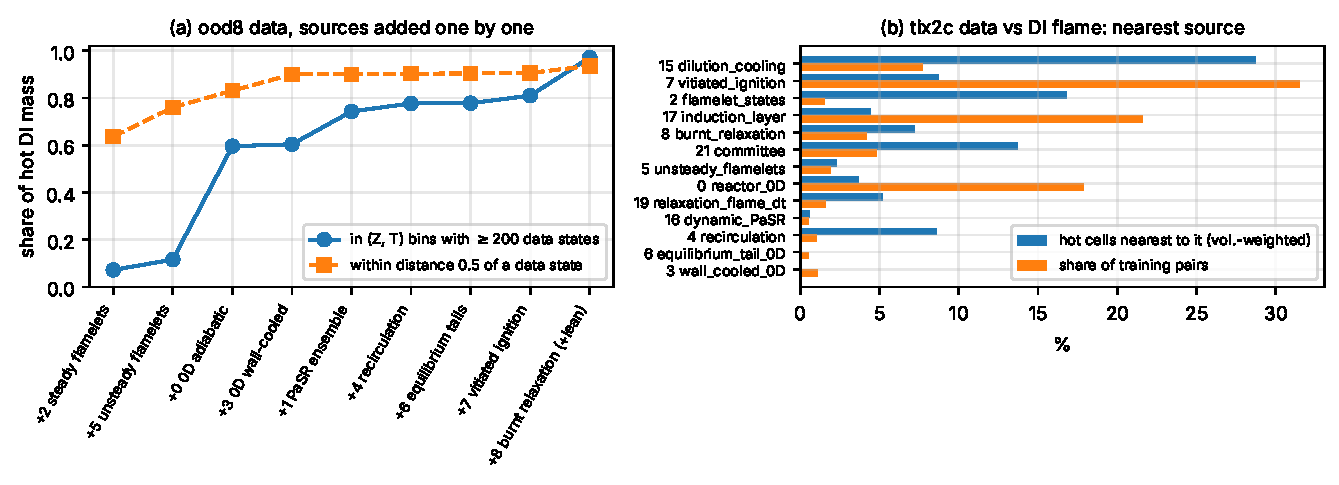
\includegraphics[width=\textwidth]{figs/fig_coverage.pdf}
\caption{(a) Share of the hot DI mass of the Fluent burner solution covered by the ood8 data as sources are added: in
$(Z,T)$ bins holding at least 200 states (dense) and within a standardised distance of 0.5. (b) For the final tix2c
data and the OpenFOAM DI reference: the share of hot cells whose nearest training state comes from each source, against
the source's share of the data.}
\label{fig:coverage}
\end{figure}

\subsection{What each source fixed in the simulation}
The sources were added one at a time, each after a coupled simulation showed a specific failure. The early steps were
made on an earlier configuration of the burner (lateral outlet, no wall radiation) and are given as development
history; the final scores are on the corrected configuration (Section~\ref{sec:cfd}).
\begin{itemize}
\item \emph{Equilibrium tails (6)}: the first network was 35~K cold in the flame core near the nozzle, inside its data,
  with OH twice and CO 1.4 times DI; the tails brought the flame error to 3--6~K (hybrid mode).
\item \emph{Vitiated ignition (7) and burnt-gas relaxation (8)}: every network ignited the jet about 1.5~ms early. The
  cause was proven by switching chemistry back to DI above a temperature threshold: the networks pumped radicals into
  the hot lean starting gas (OH 10--17 times, H about 1000 times DI), which then ignited the jet. Relaxation with
  perturbed radicals was added against the radical pumping and vitiated ignition against the induction error;
  together they were necessary but not sufficient: the network trained with both (ood8) still ignited early in
  pure mode, and only DI in the induction cells (hybrid mode) removed the error.
\item \emph{Time-step range}: training over a twentyfold wider $\Delta t$ range (\SI{1}{\micro s}--50~ms) at equal size
  raised the flame error from 3--6 to 24--57~K at the flow step; pairs must concentrate where the solver's
  $\tau_\mathrm{cell}$ distribution is.
\item \emph{Flow-informed bounds (tix2)}: cut the OOD share of the radiation-cooled lean gas from 27--61\% to 5--27\% of the
  advanced cells.
\item \emph{Hole sources and committee (tix2h, tix2c)}: the induction layer and committee states, aimed at ignition,
  improved the flame instead (14.9 to 8.0~K, OH error 23 to 10\%) and left the ignition 0.6~ms early.
\end{itemize}

\subsection{Coupled simulation}
\label{sec:cfd}
Every data family was scored with a fixed protocol in pure mode (no DI fallback) on the corrected burner: an ignition
phase from a lean start and a 50~ms window of the established flame, combined into $S=\max(F,I,C)$ with $F$ the flame
temperature error over 5~K, $I$ the ignition-delay error over 0.3~ms and $C$ the CO/OH total error over a factor 1.4
\todo{cite protocol paper}. Figure~\ref{fig:families} shows the result. Three training repeats of one data set span a
factor of 2--5 in $S$ (ood8: 4.67--14.1; tix2h: 2.35--10.6), more than the differences between data sets; the mean
ensemble of the repeats is always better than its members. The best physics-only model is the ensemble of three tix2c
networks, $S=2.00$: flame error 8.0~K with a drift of 0.5~K per 10~ms, ignition 0.6~ms early, OH and CO L1 errors 10
and 6\%, 2.6\% of flame cells OOD. Tabulation (ISAT, tolerance \num{e-4}) on the same case meets every target
($S=0.67$: 0.9~K, $-0.2$~ms) at the same cost per step.

\begin{figure}[t]
\centering
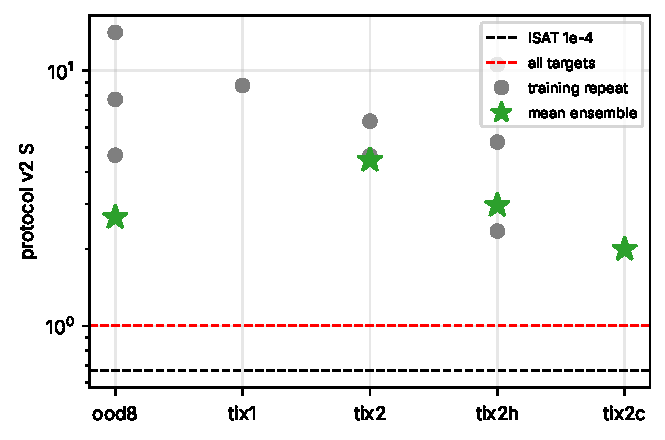
\includegraphics[width=0.6\textwidth]{figs/fig_families.pdf}
\caption{Protocol score of each physics-only data family in the coupled burner simulation: training repeats (dots) and
their mean ensemble (stars); dashed: all targets met ($S=1$) and ISAT at tolerance \num{e-4}.}
\label{fig:families}
\end{figure}

%% ===============================================================================================
\section{Discussion}
\label{sec:discussion}
\paragraph{Coverage is necessary and not sufficient} With the hole sources, every hot state of the flame is inside the
data and the solver flags almost none as OOD, yet the best network is 8~K off and ignites early. The error that
remains is precision: the induction chemistry of a few cells at the jet base, which sets the ignition delay, and the
slow recombination near equilibrium, where radical mass fractions span many decades and an absolute loss sees
little. More states in the same places will not fix it; a loss weighted towards those regions, more capacity, or
pairs at the exact time steps the solver uses might.

\paragraph{Where the data go is not where they are needed} Vitiated ignition and the induction layer make up half of
the final data and are nearest to an eighth of the flame's hot volume; dilution--cooling parcels make up 8\% and are
nearest to 29\%. Sources aimed at ignition improved the flame and not the ignition. Coverage measures on a reference
solution are the cheapest way to see this before training.

\paragraph{Diagnostics can mislead} The apparent excess-enthalpy hole was a numerical artefact of the diffusion model
of one solver; a hole map from one code must be checked against another before it changes the exploration.

\paragraph{Repeats} Because the spread between training repeats is as large as the differences between data sets,
statements of the form ``source X improved the network'' need several repeats or ensembles; the steps listed above that
rest on single networks are indications, not proofs.

\paragraph{Using the simulation without training on it} The exploration used the simulation only through flow
statistics and hole maps. An iterative loop that seeds new Cantera explorations from the states where a network fails,
still without using them as data, fixed the ignition delay but degraded the flame \todo{cite comparison paper}; online
training on the simulation's own DI pairs reached $S=1.04$ but is, by construction, no longer a physics-only model.

\paragraph{Limitations} One mechanism, one fuel, one pressure (1~atm; the network has seen no other), one laminar burner.
The approach is mechanism-agnostic, but the sources and bounds were tuned to this configuration, and the main reviewer
question will be how it transfers. \todo{second case or mechanism (a 22-species reduction of GRI-Mech 3.0 is being
explored with the same sources).}

\section{Conclusions}
\begin{enumerate}
\item A thermochemical-space exploration built only from the mechanism, the inlet streams and boundary physics, bounded
  by flow statistics, covers every hot state of a laminar methane/air burner: no hot cell of the DI solution lies
  outside the data.
\item Flamelets alone place only 7\% of the hot mass in densely sampled regions; reactor, mixing and relaxation sources
  bring this to 97\%, and burnt-gas relaxation is the one source no other replaces.
\item Each source was justified by a failure of the coupled simulation: equilibrium tails by a cold flame core,
  relaxation with perturbed radicals by an ignition triggered by radical pumping, dilution--cooling parcels by the warm
  lean gas that holds most of the hot mass.
\item Full coverage still leaves an 8~K flame error and a 0.6~ms early ignition for the best ensemble, above tabulation at
  the same cost: the remaining problem is precision, and the spread between training repeats is as large as the gain of
  any single source.
\end{enumerate}

\section*{Data and code availability}
\todo{chemmanifold-studio: chemmanifold/ (stages 0--4, holes.py, unsteady\_flamelet.py), configs/burner\_openfoam\_tix2c.yaml,
scripts/16\_coverage\_gaps.py, scripts/23\_committee\_sampling.py, papers/data/coverage/, results/sim1/.}

\section*{Acknowledgements}
\todo{}

\bibliographystyle{elsarticle-num}
\bibliography{refs}

\end{document}
